% The Clever Algorithms Project: http://www.CleverAlgorithms.com
% (c) Copyright 2011 Jason Brownlee. Some Rights Reserved. 
% This work is licensed under a Creative Commons Attribution-Noncommercial-Share Alike 2.5 Australia License.

% Name
% The algorithm name defines the canonical name used to refer to the technique, in addition to common aliases, abbreviations, and acronyms. The name is used in terms of the heading and sub-headings of an algorithm description.
\section{Stepwise Regression} 
\label{sec:stepwise}
\index{Stepwise Regression}
\index{Stepwise Multiple Linear Regression}

% other names
% What is the canonical name and common aliases for a technique?
% What are the common abbreviations and acronyms for a technique?
\emph{Stepwise Regression, Stepwise Selection, Stepwise Multiple Linear Regression}

% Taxonomy: Lineage and locality
% The algorithm taxonomy defines where a techniques fits into the field, both the specific subfields of Computational Intelligence and Biologically Inspired Computation as well as the broader field of Artificial Intelligence. The taxonomy also provides a context for determining the relation- ships between algorithms. The taxonomy may be described in terms of a series of relationship statements or pictorially as a venn diagram or a graph with hierarchical structure.
\subsection{Taxonomy}
% To what fields of study does a technique belong?
Stepwise Regression is a Model Selection method for selecting a regression model. It was originally proposed as an extension to Multiple Linear Regression called Stepwise Multiple Linear Regression. It has since been generalized to other regression models, such as Logistic Regression for Stepwise Logistic Regression.
% What are the closely related approaches to a technique?
It is considered an improvement over Model Selection methods for Regression such as All Subsets.
It is related to other Model Selection methods for Regression such as Ridge Regression. It is also related to Regularized Regression methods such as LASSO and the Least Angle Regression used to solve it.

% Strategy: Problem solving plan
% The strategy is an abstract description of the computational model. The strategy describes the information processing actions a technique shall take in order to achieve an objective. The strategy provides a logical separation between a computational realization (procedure) and a analogous system (metaphor). A given problem solving strategy may be realized as one of a number specific algorithms or problem solving systems. The strategy description is textual using information processing and algorithmic terminology.
\subsection{Strategy}
% What is the information processing objective of a technique?
The information processing objective of the technique is to result in a regression model that minimizes a specified measure, hypothesis test or criterion, for example F-tests in the original description, or more simply here as the minimum Sum Squared Residuals (SSR).
% What is a techniques plan of action?
This achieved by a greedy hill-climbing algorithm that successively adds one of the remaining variables to the regression model that result in the largest reduction in the SSR and then refits the model. The procedure stops once no further improvements to the specified criterion can be achieved or there are no more variables to add to the model. This process alone is called Forward Model Selection. Conversely, the greedy algorithm may start with all variables and successively remove one that result in the largest decrease in the SSR. This approach alone is called Backward Selection.

Stepwise Regression applies Forward Model Selection as well as Backward Model Selection, allowing variables that have become redundant through the addition of other variables, to be removed from the model later in the process. The procedure requires the specification of threshold parameters for the minimum change in the of the selected measure for adding (F-to-enter) and removing (F-to-remove) variables to and from the model. The Forward method is applied until it can no longer add any more variables, then the Backward method is applied. This sequence repeats until the model stabilizes. One may start with no variables and successively grow a model, called Forward Stepwise Regression, or start with all variables and successively prune the model, called Backward Stepwise Regression.

% Heuristics: Usage guidelines
% The heuristics element describe the commonsense, best practice, and demonstrated rules for applying and configuring a parameterized algorithm. The heuristics relate to the technical details of the techniques procedure and data structures for general classes of application (neither specific implementations not specific problem instances). The heuristics are described textually, such as a series of guidelines in a bullet-point structure.
\subsection{Heuristics}
% What are the suggested configurations for a technique?
% What are the guidelines for the application of a technique to a problem instance?
\index{Akaike Information Criterion}
\index{AIC}
\index{Bayes Information Criterion}
\index{BIC}

\begin{itemize}
	\item Given the greedy nature of the selection procedure, neither Forward nor Backward Stepwise Regression generally result in the selection of optimum model, but rather a sub-optimal modal that is commonly close to the optimum model.
	\item It is typically applied to Linear Regression and Generalized Linear Regression Models.
	\item Modern implementations use Hypothesis based tests between models (such as a t-test or an F-test) or criteria-based tests such as the Akaike Information Criterion (AIC) and the Bayes Information Criterion (BIC).
	\item Criterion tests for adding and removing variables such as AIC and BIC are preferred over hypothesis-based tests (such as the F-test) as the use of the latter have been discredited \cite{Pope1972, Wilkinson1979}.
	\item If the errors are normally distributed, the Akaike Information Criterion (AIC) selection criteria can be used \cite{Akaike1973}.
	\item Using a cross-validated error score for making decisions to add and remove variables may result in an improved final model.
	\item Resulting models frequently fail to include all variables that have an influence on the dependent variable while also frequently including variables that do not influence the dependent variable \cite{Derksen1992}, meaning the final model is generally not the best model \cite{Miller1984} (taken from \cite{Mundry2009}).
	\item 
\end{itemize}

% sample script in R
\subsection{Code Listing}
% listing
Listing~\ref{stats_stepwise_linear_regression} provides a code listing of Stepwise Multiple Linear Regression method in R. Figure~\ref{plot:stepwise_regression_result} provides a plot of the training dataset with the line of best fit highlighted.

% algorithm and package
The example uses the {lm()} function and the and \texttt{step()} in the \texttt{stats} core package which are responsible for fitting linear models and performing stepwise selection respectively. The \texttt{step()} function uses a Akaike Information Criterion as the model evaluation criteria.

% problem
The test problem is a four-dimensional dataset of 100 samples, where the \texttt{x1}, \texttt{x2}, \texttt{x3} values are drawn from a uniformly random distribution $x \in [0,10]$ and \texttt{y} values are dependent on the \texttt{x1} value plus a value drawn from a normally random distribution with a mean of 0 and a standard deviation of 1. The features \texttt{x2} and \texttt{x3} are random independent variables that have no relevant interaction \texttt{x1} and \texttt{y}. In this example, \texttt{y} is considered the dependent variable and \texttt{x1} the single relevant independent. The stepwise method is expected to discount \texttt{x2} and \texttt{x3} and select a linear model for \texttt{y} given \texttt{x1}.

\lstinputlisting[firstline=7,language=r,caption={Example of Stepwise Multiple Linear Regression in R using the \texttt{lm()} and \texttt{step()} functions in the \texttt{stats} core package.}, label=stats_stepwise_linear_regression]{../src/algorithms/regression/stats_stepwise_linear_regression.R}

\begin{figure}[htp]
\centering
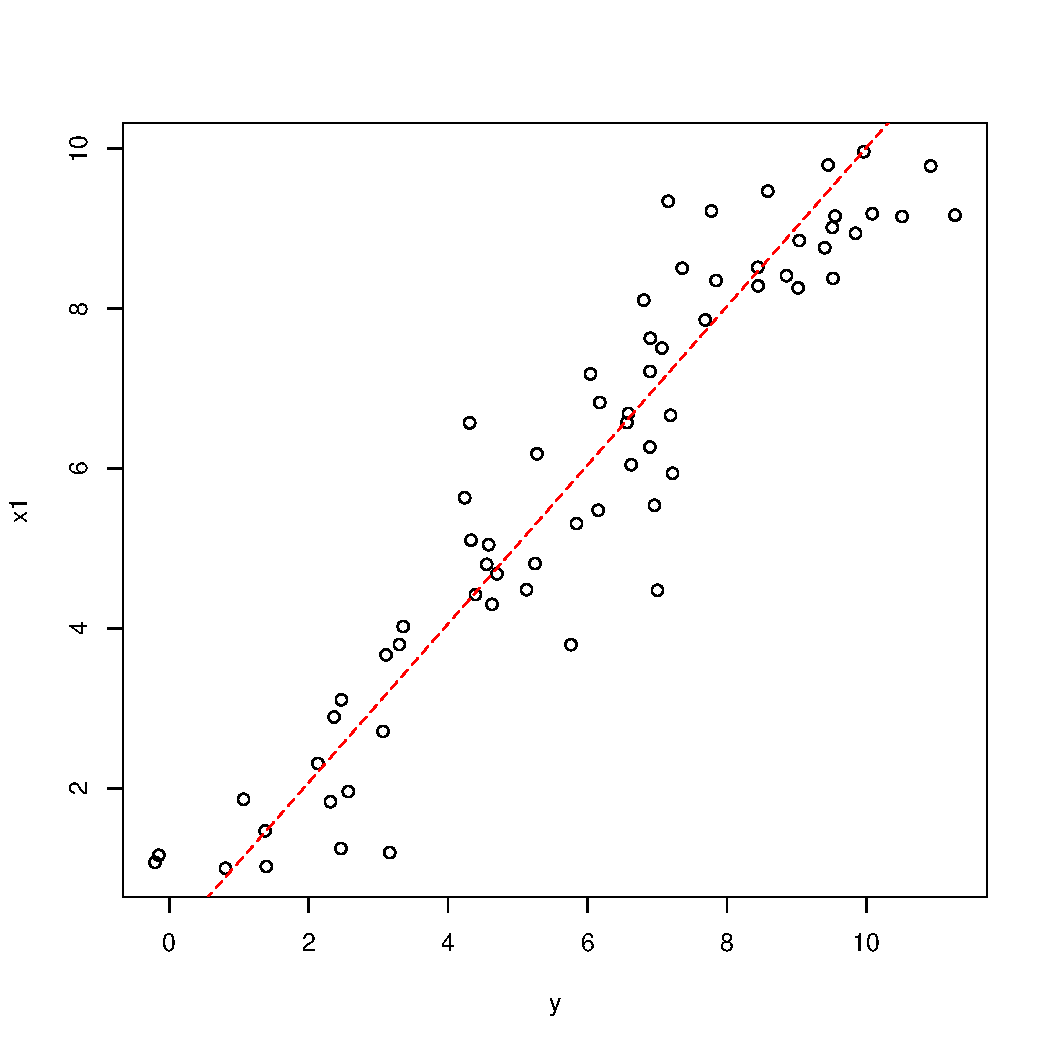
\includegraphics[scale=0.45]{a_regression/stepwise_regression_result.pdf}
\caption{Plot 2D training dataset with the line of best fit.}
\label{plot:stepwise_regression_result}
\end{figure}

% other packages
Other packages that provide stepwise selection include the \texttt{stepAIC} function of the \texttt{MASS} package. The \texttt{leaps} package does not provide stepwise selection, although does provides a related selection method called Regression Subset Selection that uses a branch and bound search.

% References: Deeper understanding
% The references element description includes a listing of both primary sources of information about the technique as well as useful introductory sources for novices to gain a deeper understanding of the theory and application of the technique. The description consists of hand-selected reference material including books, peer reviewed conference papers, journal articles, and potentially websites. A bullet-pointed structure is suggested.
\subsection{References}
% What are the primary sources for a technique?
% What are the suggested reference sources for learning more about a technique?

% primary sources
\subsubsection{Primary Sources}
% seminal
Efroymson is credited with Stepwise Multiple Linear Regression in which he used F-test significance for the add and remove decisions \cite{Efroymson1960}.
% early review
Breaux provides an early and salient overview of Efroymson's Stepwise Multiple Regression in his technical report that promotes the method as computationally efficient over enumerating all subsets of regression models \cite{Breaux1967}.

% more info
\subsubsection{More Information}
% general references
Hocking provides an early and detailed review of forward and backward variable selection methods and of Stepwise Multiple Linear Regression \cite{Hocking1976}.
Miller provides an analysis on the convergence of Stepwise Regression \cite{Miller1996}.
% stepwise is a bad idea
Whittingham et~al.\ provide a modern enumeration of all of the known problems and reasons against using Stepwise Multiple Regression for modelling, and fret about its commonplace use in the field ecology \cite{Whittingham2006}.
Mundry and Nunn provide a similar review and focus on the limitations of the meod for statistical inference \cite{Mundry2009}.
% usage in R
Faraway provides a good example of Stepwise procedures for regression with examples in R \cite{Faraway2002} (page 125).


% END
